\def\mytitle{Assignment-Gate 2011 EC Q20}
\def\mykeywords{}
\def\myauthor{Nikhil Nair}
\def\contact{}
\def\mymodule{Future Wireless Communication}
\documentclass[10pt, a4paper]{article}
\usepackage[a4paper,outer=1.5cm,inner=1.5cm,top=1.75cm,bottom=1.5cm]{geometry}
\twocolumn
\usepackage{graphicx}
\graphicspath{{./images/}}
\usepackage[colorlinks,linkcolor={black},citecolor={blue!80!black},urlcolor={blue!80!black}]{hyperref}
\usepackage[parfill]{parskip}
\usepackage{lmodern}
\renewcommand*\familydefault{\sfdefault}
\usepackage{watermark}
\usepackage{karnaugh-map}
\usepackage{lipsum}
\usepackage{xcolor}
\usepackage{listings}
\usepackage{float}
\usepackage{titlesec}
\usepackage{amsmath}
\usepackage{algorithm2e}

\titlespacing{\subsection}{0pt}{\parskip}{-3pt}
\titlespacing{\subsubsection}{0pt}{\parskip}{-\parskip}
\titlespacing{\paragraph}{0pt}{\parskip}{\parskip}
\newcommand{\figuremacro}[5]{
    
}

\lstset{
frame=single, 
breaklines=true,
columns=fullflexible
}
\thiswatermark{\centering \put(0,-105.0){
\includegraphics[scale=0.5]{iith.png}} }
\title{\mytitle}
\author{\myauthor\hspace{1em}\\\contact\\IITH\hspace{0.5em}-\hspace{0.5em}\mymodule}
\date{}
\hypersetup{pdfauthor=\myauthor,pdftitle=\mytitle,pdfkeywords=\mykeywords}
\sloppy
\begin{document}
  \maketitle
\tableofcontents



\section{Components}



\begin{table}[htbp]
 \begin{center}
    \begin{tabular}{|l|c|c|c|c|c|c} \hline \textbf{Component}
  & \textbf{Value} & \textbf{Quantity} \\
 \hline
Resistor & 220 ohm & 1 \\ \hline
Arduino & UNO & 1 \\ \hline
Decoder & 7447 & 1 \\ \hline
Display &  & 1 \\ \hline
Bread board &  & 1 \\ \hline
Jumper wires & M-M & 15\\ \hline
\end{tabular}   
\end{center}
\caption{\label{table:dummytable} }
\end{table}

\section{Connections}



Make connections between Seven segment and 7447 IC as per  table3. 

\begin{table}[htbp]
 \begin{center}
    \begin{tabular}{|l|c|c|c|c|c|c|c|c} \hline \textbf{7447}
  & \textbf{a'} & \textbf{b'} & \textbf{c'}& \textbf{d'}& \textbf{e'}& \textbf{f'}& \textbf{g'} \\
 \hline
 \textbf{Display}
  & \textbf{a} & \textbf{b} & \textbf{c}& \textbf{d}& \textbf{e}& \textbf{f}& \textbf{g} \\\hline

\end{tabular}   
\end{center}
\caption{\label{table:dummytable} }
\end{table}

Make connections between Arduino and 7447 IC as per table4.


\begin{table}[htbp]
 \begin{center}
    \begin{tabular}{|l|c|c|c|c|c|c|c|c} \hline \textbf{Arduino}
  & \textbf{2} & \textbf{3} & \textbf{4}& \textbf{5} \\
 \hline
 \textbf{7447}
  & \textbf{A} & \textbf{B} & \textbf{C}& \textbf{D} \\
 \hline
 
\end{tabular}   
\end{center}
\caption{\label{table:dummytable} }
\end{table}


\section{Problem}
The logic function implemented by the circuit given below is that of an XOR Gate

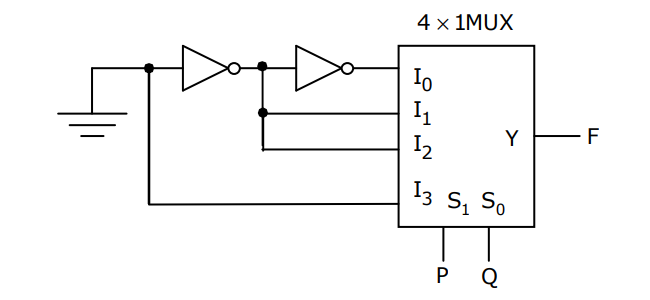
\includegraphics[scale=0.4]{cct.png}
\begin{center}
F = PQ'+ P'Q
\end{center}
        
\section{Truth table}
.
\begin{table}[htbp]
 \begin{center}
    \begin{tabular}{|l|c|c|c|c|c|c|c|c} \hline \textbf{P}
  & \textbf{Q} & \textbf{F} \\
 \hline
        0&0&0 \\
        \hline
        0&1&1 \\
        \hline
        1&0&1 \\
        \hline
        1&1&0 \\
        \hline
     
\end{tabular}   
\end{center}
\caption{\label{table:dummytable} }
\end{table}




\section{Karnaugh-map}
 \begin{center}
        \begin{karnaugh-map}[2][2][1][$Q$][$P$]
        \minterms{1,2}
        \maxterms{0,3}
      %  \implicant{1}{2}
        
        \end{karnaugh-map}

        
F = PQ'+ P'Q

\end{center}







\section{Code Link}
 Execute the following program to realize the Boolean logic for the given circuit
\vspace{5mm}
\begin{lstlisting}
https://github.com/nikhilnair90/FWC-2/blob/5c950fc2f1024337a2e919db7235bcad72a67800/Assignment%20Ide/Codes/gate2011_EC_Q20.cpp
\end{lstlisting}





\end{document}